\documentclass[journal,12pt,twocolumn]{article}
\usepackage[top = 1in,bottom = 1in,left = 1in,right = 1in]{geometry}
\setlength{\columnsep}{2cm}
\usepackage{amssymb}
\usepackage{amsfonts}
\usepackage{amsmath}
\usepackage{amsthm}
\usepackage{setspace}
\usepackage{longtable}
\usepackage{enumitem}
\usepackage{mathtools}
\usepackage{color}                                  
\usepackage{array}
\usepackage{calc} 
\usepackage{bm}
\usepackage{caption}
\usepackage{float}
%has mini page
%to fix position (H)

\setlength{\parindent}{0pt}
%no indentation for paragraphs


\newcommand{\giveneq}{x^{2}-3y^{2}-4x=8}
\newcommand{\generaleqa}{\frac{X^2}{a^2} - \frac{Y^2}{b^2} = 1}
\newcommand{\generaleqb}{-\frac{X^2}{a^2} + \frac{Y^2}{b^2} = 1}
\newcommand{\subtitute}[2]{\frac{X^2}{(#1)^2} - \frac{Y^2}{(#2)^2} = 1}
\begin{document}

\title{ASSIGNMENT-2}
\author{MUKUNDA REDDY AI21BTECH11021}
\date{}
\maketitle

\section*{\Large{Question 4(b)}}
Find the coordinates of the center,foci and equation of
the directrix of the hyperbola
$x^{2}-3y^{2}-4x=8$?\\
 \hline
\section*{Solution}
Here we should observe that there is no $xy$ term in the
given hyperbola equation so this can be converted to the
general form of hyperbola $$\generaleqa   \text{\LARGE$/$} \generaleqb$$\\

$\implies x^2-3y^2-4x = 8$\\
$\implies x^2-4x+4-3y^2 = 8+4$\\
$\implies (x-2)^2-3y^2 = 12$\\
\begin{equation}
\implies \frac{(x-2)^2}{12}-\frac{y^2}{4} = 1
\end{equation}

Applying transformation to convert into standard form
subtitute $X=x-2$ and $Y = y$ $$\implies \subtitute{12}{4} $$
It takes the first general form so transverse axis is parallel
to $x-axis$ and conjugate axis is parallel to $y-axis$.

\begin{table}[t]
    \centering
    \hline
    \renewcommand{\arraystretch}{2}
    \begin{tabular}{|p{2.2cm}|p{1.2cm}|p{1.2cm}|p{1.7cm}|}
    $\generaleqa$  & Center & Foci & Directrix equation\\ \hline
      Location  &   $(0,0)$ & $(\pm ae,0)$ & $X=\pm \frac{a}{e}$\\ \hline
    \end{tabular}
    \caption*{properties}
\end{table}

Here $e$ is called eccentricity of hyperbola defined as

\begin{equation}
\label{eccentricity}
 e=\sqrt{1+\frac{b^2}{a^2}} 
\end{equation}

From \eqref{eccentricity} we have $a^2 = 12 , b^2 = 4$.
$$\implies e = \sqrt{1+\frac{4}{12}}=\sqrt{\frac{4}{3}}=\frac{2}{\sqrt{3}}$$
  \subsection*{Center of hyperbola}
  center of $\generaleqa$ is $(X,Y) = (0,0)$.As $X = x-2$ and $Y = y$
  we have center of $ \generaleq $ that is $(x,y) = (2,0)$ \\
  
  \subsection*{Foci of hyperbola}
  foci of $\generaleqa$ is $(X,Y) = (\pm ae,0)$.
  \begin{align*}
  \implies Y &= y = 0\\
  \implies X &= \pm ae = \pm 2\sqrt{3} * \cfrac{2}{\sqrt{3}}\\
  \implies X &= \pm 4 \\
  \implies x &= X+2 = \pm 4 + 2\\
  \implies x &= 6 \; \text{or} -2\\  
  \end{align*}
  \therefore \text{foci of hyperbola }$(x,y) = (6,0) \text{ and } (-2,0)$ \\
  \pagebreak

\subsection*{Directrix of hyperbola}
   For the general equation $$\generaleqa$$ It is
   given by X = $\pm \frac{a}{e}$\\
   \columnbreak
  \begin{align*}
      \implies X &= \pm \cfrac{2\sqrt{3}}{\cfrac{2}{\sqrt{3}}} \\
      \columnbreak
      \implies X &= \pm \sqrt{3}*\sqrt{3} = 3 \\
      \implies x &= X+2 = \pm3+2\\
      \implies x &= 5 \text{ or } -1\\
  \end{align*}
  \therefore \text{Directrix of hyperbola are}\\
     $$x=5 \text{ and } x = -1$$\\
     


\begin{figure}[H]
    \centering
    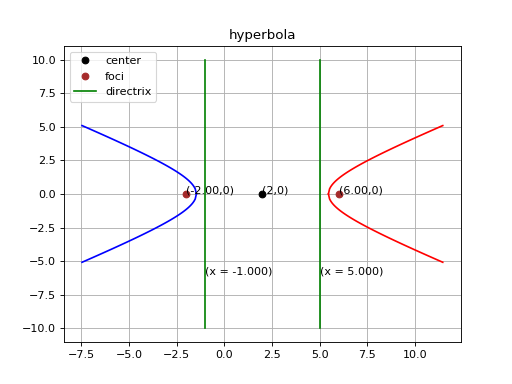
\includegraphics[scale=1.05]{hyperbola.png}
    \label{fig:my_hyperbola}
\end{figure}

\begin{figure}[H]
    \centering
    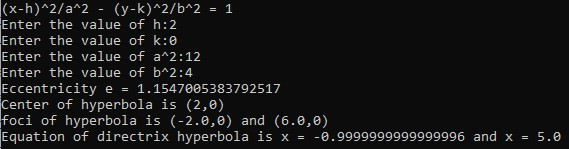
\includegraphics[scale=1]{pythoncode.jpg}
    \caption*{Verification}
    \label{fig:my_code}
\end{figure}

\end{document}
